\documentclass[border=10pt]{standalone}

\usepackage{tikz}
\usepackage{tikzsymbols}
\usetikzlibrary{calc,patterns,shapes.geometric}

\def\centerarc[#1](#2)(#3:#4:#5){\draw[#1] ($(#2)+({#5*cos(#3)},{#5*sin(#3)})$) arc (#3:#4:#5);}

\begin{document}
	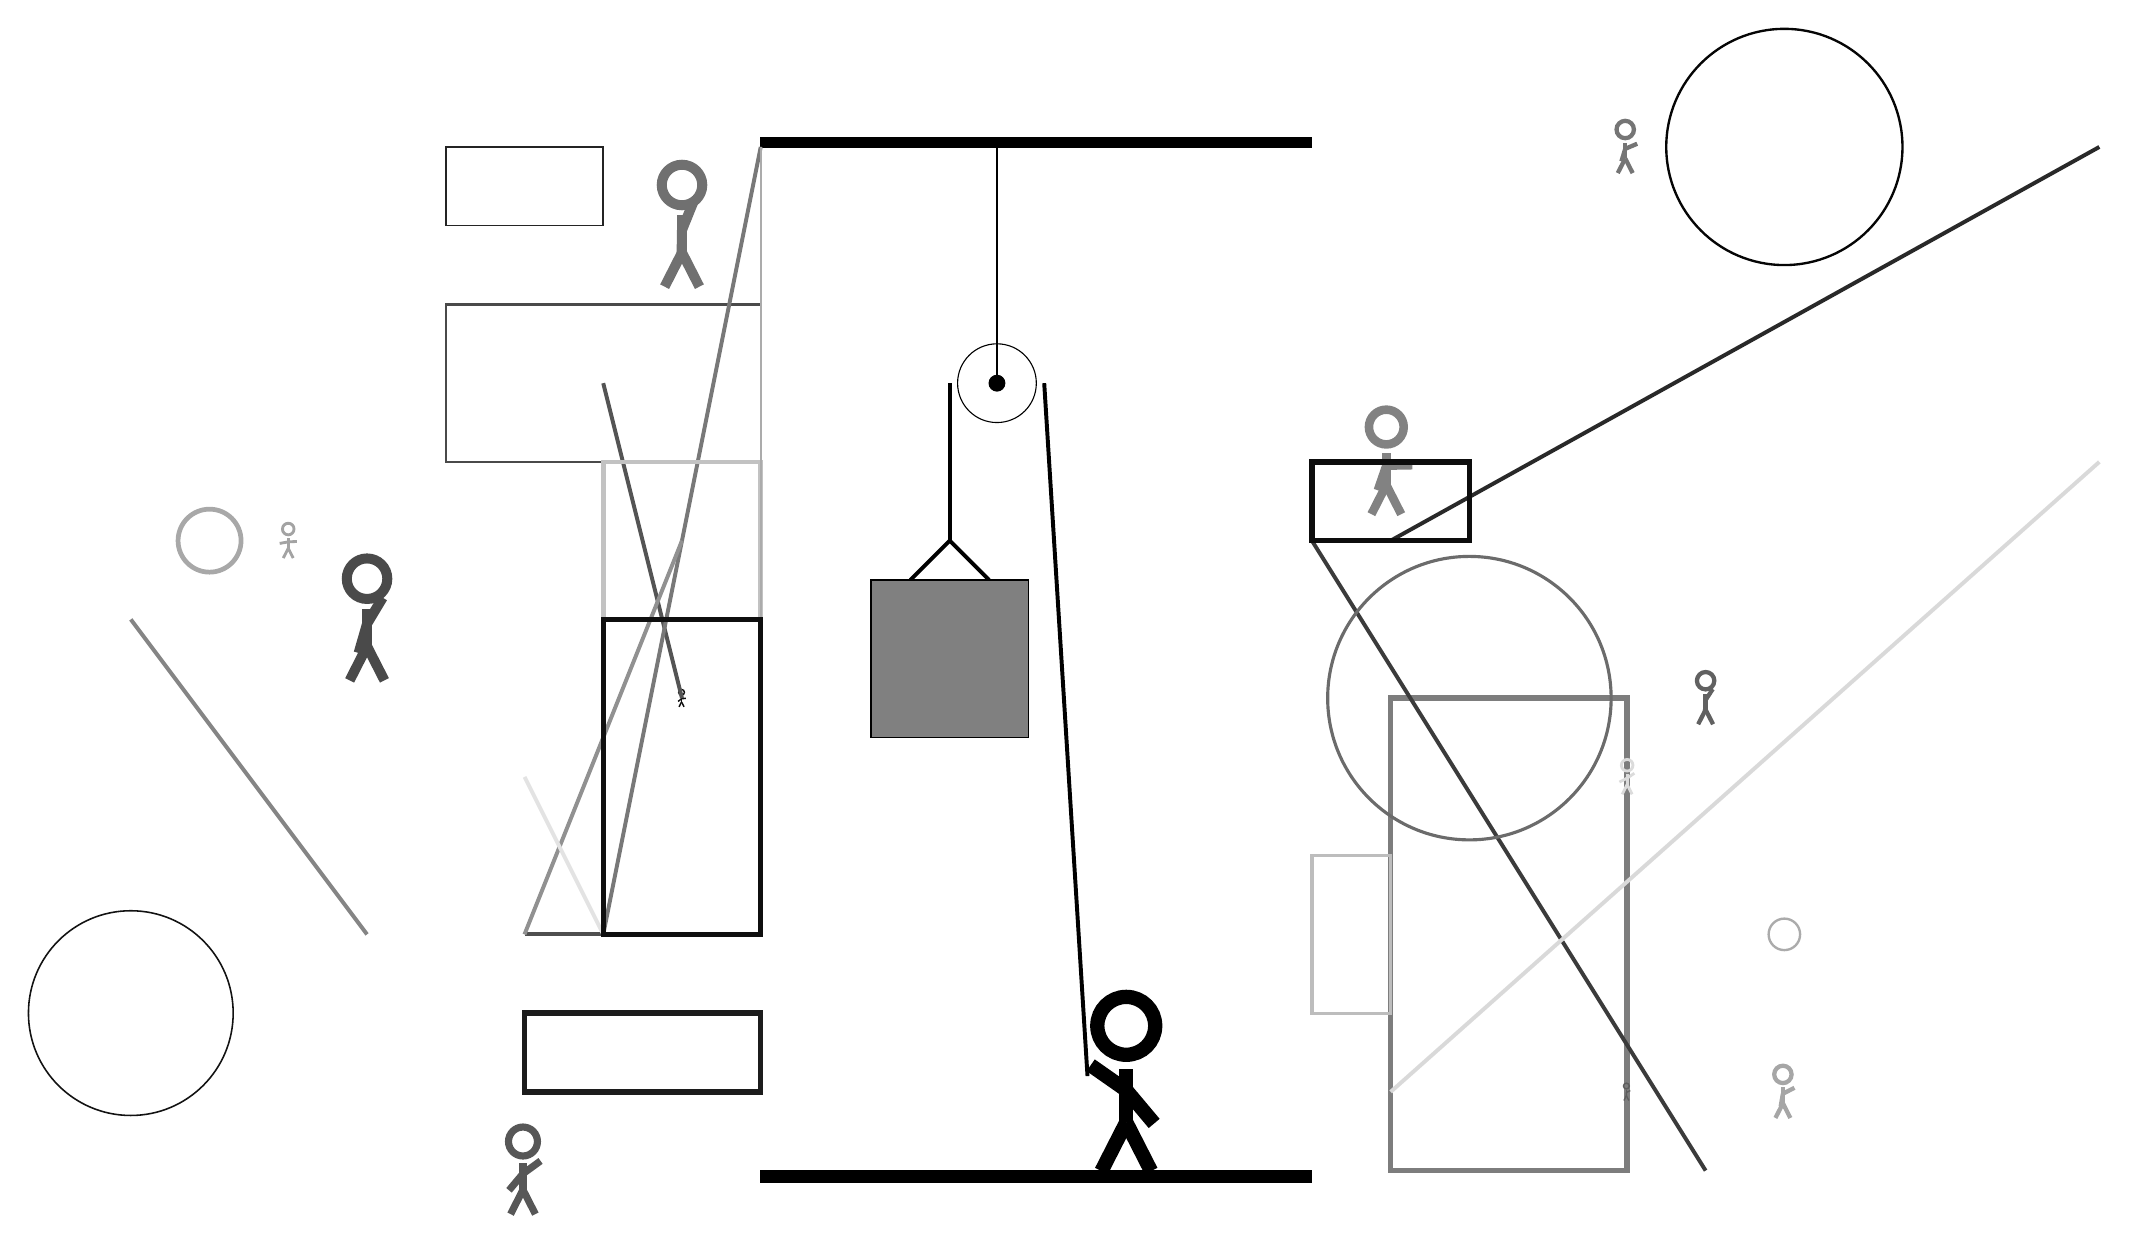
\begin{tikzpicture}
		%%%%% START %%%%%
		
		\draw[fill=black] (-2, 10) rectangle (5, 10.125);
		
		\draw[line width=0.7mm, color=black!51] (6, 3) rectangle (9, -3);
		
		\draw [line width=0.3mm, color=black!98](11, 10) circle (1.5);
		\draw [line width=0.6mm, color=black!34](-9, 5) circle (0.4);
		\node[line width=0.7mm, color=black!36] at (-8, 5) {\Strichmaxerl[2][10][3]};
		\node[line width=0.6mm, color=black!49] at (6, 6) {\Strichmaxerl[6][71][1]};
		\node[line width=0.7mm, color=black!94] at (-3, 3) {\Strichmaxerl[1][38][6]};
		\draw[line width=0.5mm, color=black!77](10, -3) -- (5, 5);
		\node[line width=0.4mm, color=black!71] at (-7, 4) {\Strichmaxerl[7][74][59]};
		\draw[line width=0.5mm, color=black!67](-3, 3) -- (-4, 7);
		
		\draw[line width=0.5mm, color=black!84](6, 5) -- (15, 10);
		\node[line width=0.6mm, color=black!14] at (9, 2) {\Strichmaxerl[2][27][34]};
		
		\node[line width=0.7mm, color=black!62] at (10, 3) {\Strichmaxerl[3][87][57]};
		\node[line width=0.5mm, color=black!66] at (-5, -3) {\Strichmaxerl[5][50][36]};
		\draw[line width=0.5mm, color=black!15](6, -2) -- (15, 6);
		\draw[line width=0.3mm, color=black!71] (-2, 8) rectangle (-6, 6);
		\draw[line width=0.5mm, color=black!69](-5, 0) -- (-4, 0);
		
		\draw[line width=0.5mm, color=black!53](-2, 10) -- (-4, 0);
		\draw[line width=0.6mm, color=black!24] (-2, 6) rectangle (-4, 4);
		\draw[line width=0.2mm, color=black!86] (-4, 9) rectangle (-6, 10);
		
		\draw[line width=0.2mm, color=black!33] (-2, 10) rectangle (-2, 3);
		\draw [line width=0.4mm, color=black!58](7, 3) circle (1.8);
		
		\draw[line width=0.7mm, color=black!95] (7, 6) rectangle (5, 5);
		
		\draw [line width=0.3mm, color=black!41](7, 7) circle (0.0);
		\draw [line width=0.2mm, color=black!93](-10, -1) circle (1.3);
		\node[line width=0.2mm, color=black!56] at (-3, 9) {\Strichmaxerl[7][89][68]};
		\draw[line width=0.7mm, color=black!89] (-2, -1) rectangle (-5, -2);
		\draw[line width=0.5mm, color=black!43](-5, 0) -- (-3, 5);
		\draw [line width=0.3mm, color=black!33](11, 0) circle (0.2);
		\draw[line width=0.5mm, color=black!11](-4, 0) -- (-5, 2);
		\draw[line width=0.7mm, color=black!94] (-4, 0) rectangle (-2, 4);
		\node[line width=0.2mm, color=black!35] at (11, -2) {\Strichmaxerl[3][80][27]};
		
		\draw[line width=0.4mm, color=black!26] (5, 1) rectangle (6, -1);
		\draw[line width=0.5mm, color=black!48](-7, 0) -- (-10, 4);
		\node[line width=0.3mm, color=black!54] at (9, 10) {\Strichmaxerl[3][73][23]};
		\node[line width=0.7mm, color=black!63] at (9, -2) {\Strichmaxerl[1][88][26]};
		
		\draw (1, 7) circle (0.5);
		\draw[fill=black] (1, 7) circle (0.1);
		\draw (1, 10) -- (1, 7);
		
		\draw[line width=0.5mm] (-0.1, 4.5) -- (0.4, 5.0) -- (0.9, 4.5);
		\draw[fill=black!50] (-0.6, 4.5) rectangle (1.4, 2.5);
		
		\draw[line width=0.5mm] (0.4, 7) -- (0.4, 5.0);
		\centerarc[line width=0.5mm](1, 7)(0:180:0.6);
		\draw[line width=0.5mm](1.6, 7) -- (2.15, -1.8);
		
		\node at (2.6, -1.9) {\Strichmaxerl[10][-35][-50]};
		
		\draw[fill=black] (-2, -3) rectangle (5, -3.15);
		
		%%%%% END %%%%%
	\end{tikzpicture}
\end{document}